%\begin{myact}{1 Différentes écritures des nombres}
%
%	\label{act:nbres}
%	
%	\begin{enumerate}
%		\item Donner deux nombres à 2, 3, 4 et 5 chiffres.
%		
%		%\item \'Ecrire les nombres suivants en toutes lettres : \num{32}, \num{128} et \num{1024}. 
%		\item \'Ecrire  le nombre 25146041337 en séparant les classes.
%		\item La planète Mars a un rayon d'environ \textbf{3,4 milliers} de km, une superficie d'environ \textbf{144,8 millions} de $km^2$ et un volume d'environ \textbf{163 milliards} de $km^3$.
%		
%		\'Ecrire les trois nombres en gras en utilisant que des chiffres.
%		
%		\item Lire le texte ci-dessous, puis écrire en chiffres les nombres en gras.
%		
%			\begin{center}
%				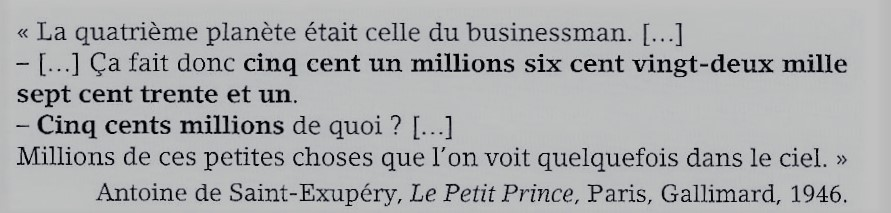
\includegraphics[scale=1.1]{img/act1}
%			\end{center}
%	\end{enumerate}
%\end{myact}

%\begin{myactrep}{1 Différentes écritures des nombres}
	
%	\begin{enumerate}
%		\item 
%			\begin{itemize}
%				\item 17 et 42 sont des nombres à 2 chiffres;
%				\item 128 et 512 sont des nombres à 3 chiffres;
%				\item \num{2048} et \num{4096} sont des nombres à 4 chiffres;
%				\item \num{16384} et \num{65536} sont des nombres à 5 chiffres.
%			\end{itemize}
%		
%		%\item \'Ecrire les nombres suivants en toutes lettres : \num{32}, \num{128} et \num{1024}. 
%		\item Le nombre 25146041337 s'écrit \num{25146041337}.
%		\item 
%			\begin{itemize}
%				\item 3,4 milliers s'écrit \num{3400};
%				\item 144,8 millions s'écrit \num{144800000};
%				\item 163 milliards s'écrit \num{163000000000}.
%			\end{itemize}
%		
%		\item .
%			\begin{itemize}
%				\item Cinq-cent-un-millions-six-cent-vingt-deux-mille-sept-cent trente-et-un s'écrit \num{501622731};
%				\item Cinq-cent-millions s'écrit \num{500000000}.
%			\end{itemize}
%
%	\end{enumerate}
%\end{myactrep}


\begin{mydef}
	\begin{itemize}
		\item Il existe 10 \kw{chiffres} : 
		\iftoggle{eleve}{%
			\iftoggle{dys}{%
				0, 1, 2, 3, 4, 5, 6, 7, 8 et 9.	
			}{
		}
		}{%
			0, 1, 2, 3, 4, 5, 6, 7, 8 et 9.	
		}
		
		\item On utilise les chiffres pour  
		\iftoggle{eleve}{%
			\iftoggle{dys}{%
				écrire des	nombres
			}{
			}
		}{%
			écrire des nombres
		}.
		
		
	\end{itemize}
\end{mydef}

\begin{myexs}
	\begin{enumerate}
		\item Quels nombres peut-on écrire avec les chiffres  2 et 4 ?
		
		\iftoggle{eleve}{%
			\iftoggle{dys}{%
				On peut écrire les nombres 
			}{
				\vspace*{0.5cm}
			}
		}{%
			On peut écrire les nombres 24 et 42.
		}
		
		\item Le nombre \num{49096} s'écrit avec quels chiffres ? 
		
		\iftoggle{eleve}{%
			\iftoggle{dys}{%
				Il s'écrit avec les chiffres 4, 0, 9 et 6.
			}{
				\vspace*{0.5cm}
			}
		}{%
			Il s'écrit avec les chiffres 4, 0, 9 et 6.
		}
		
		
	\end{enumerate}
\end{myexs}





\begin{mydefs}
	\begin{itemize}
		\item Pour mieux lire un grand nombre, on regroupe \iftoggle{eleve}{%
			\iftoggle{dys}{%
				 ses chiffres en classes par groupe de 3.
			}{
				\vspace*{0.75cm}
			}
		}{%
			 ses chiffres en classes par groupe de 3.
		}
		
		\item Un \kw{nombre décimal} possède \iftoggle{eleve}{%
			\iftoggle{dys}{%
				une \kw{partie entière} (avant la virgule) et une \kw{partie décimale} (après la virgule).
			}{
				\vspace*{0.75cm}
			}
		}{%
			une \kw{partie entière} (avant la virgule) et une \kw{partie décimale} (après la virgule).
		}
		
		\item Un \kw{nombre entier} est un nombre décimal où 
		\iftoggle{eleve}{%
			\iftoggle{dys}{%
				 la partie décimale ne contient que des zéros. Dans ce cas la partie décimale n'apparait pas.
			}{
				\vspace*{0.75cm}\\
				Dans ce cas la partie décimale n'apparait pas.
			}
		}{%
			 la partie décimale ne contient que des zéros. Dans ce cas la partie décimale n'apparait pas.
		} 
		
	\end{itemize}
\end{mydefs}

\begin{center}
	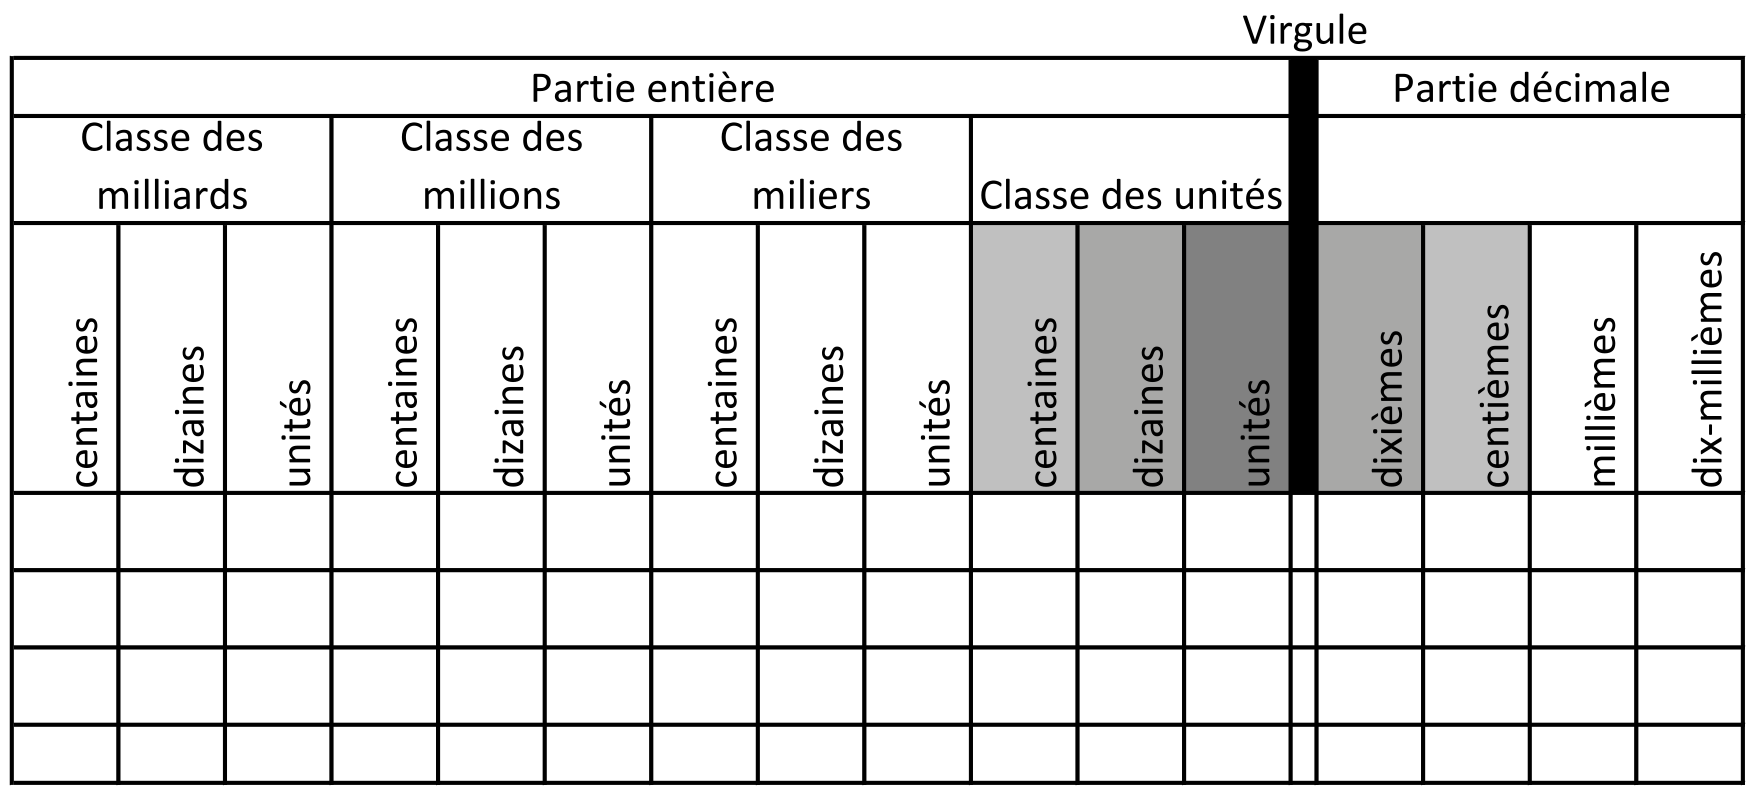
\includegraphics[scale=0.34]{img/tab_rangs}
\end{center}

\begin{myexs}
	\begin{enumerate}
		\item \'Ecrire correctement le nombre 1845937126 :
		
		\iftoggle{eleve}{%
			\iftoggle{dys}{%
				Ce nombre s'écrit 
			}{
				\vspace*{1cm} %\ \\
				
			}
		}{%
			Ce nombre s'écrit \num{1845937126}.
		} 
		
		%\item Le nombre \num{2048} est un nombre entier.
		\item Donner la partie entière et la partie décimale de  \num{5239.67} :
		
		\iftoggle{eleve}{%
			\iftoggle{dys}{%
				La partie entière de   \num{5239.67} est \hspace*{3cm} et sa partie décimale est 	
			}{
				\vspace*{1cm} %\ \\
				
			}
		}{%
			La partie entière de   \num{5239.67} est \num{5239} et sa partie décimale est 67.	
		}
	
		
		
		
		
		\item Donner le chiffre des centaines et le nombre de dizaines de \num{1337}.
		
		
		\iftoggle{eleve}{%
			\iftoggle{dys}{%
				Dans \num{1337}, le chiffre des centaines est \hspace*{2cm} et le nombre de dizaines est \hspace*{2cm}.
			}{
				\vspace*{1cm} %\ \\
				
			}
		}{%
			Dans \num{1337}, le chiffre des centaines est 3 et le nombre de dizaines est 133.
		}
		
		
		\item Donner une autre écriture possible du nombre 124 :
		
		\iftoggle{eleve}{%
			\iftoggle{dys}{%
				Le nombre entier \num{124} peut aussi s'écrire 
			}{
				\vspace*{1cm} %\ \\
				
			}
		}{%
			Le nombre entier \num{124} peut aussi s'écrire \num{124.00}.
		}
	

	\end{enumerate}
\end{myexs}


\begin{mymethname}{\'Ecrire un nombre en toutes lettres}
	\begin{itemize}
		\item Tous les mots qui désignent un nombre sont invariables, sauf <<vingt>> et <<cent>>;
		\item Les mots <<milliard>>, <<million>>, <<dixième>> ne désignent pas des nombres, ils prennent un <<s>> au pluriel;
		\item 80 s'écrit <<quatre-vingts>> sauf s'il est suivi d'un autre nombre;
		\item 100 s'écrit <<cents>> s'il est multiplié et non suivi d'un autre nombre, dans les autres cas il ne prend pas de <<s>>;
		\item On écrit un trait d'union entre chaque mot d'un nombre.
	\end{itemize}
\end{mymethname}

\begin{myexs}
	
	\iftoggle{eleve}{%
		\begin{itemize}
			\item 180 s'écrit %\pause <<cent-quatre-vingts>>;\pause
			\item \num{1300} s'écrit %\pause <<mille-trois-cents>>;\pause
			\item \num{4025035} s'écrit %\pause <<quatre-millions-vingt-cinq-mille-trente-cinq>>;
			\item \num{134.25} s'écrit %\pause <<cent-trente-quatre unités vingt-cinq centièmes.
		\end{itemize}
	}{%
		\begin{itemize}
			\item 180 s'écrit \pause <<cent-quatre-vingts>>;\pause
			\item \num{1300} s'écrit \pause <<mille-trois-cents>>;\pause
			\item \num{4025035} s'écrit \pause <<quatre-millions-vingt-cinq-mille-trente-cinq>>;
			\item \num{134.25} s'écrit \pause <<cent-trente-quatre unités vingt-cinq centièmes.
		\end{itemize}
	}
	
\end{myexs}

%\begin{myexos}
%	\begin{itemize}
%		\item Exercices 1 et 2 page 16 : identifier les chiffres d'un rang donné;
%		\item \Exo{4}{16} : décomposition d'un nombre;
%		\item \Exo{7}{16} : \'ecriture décimale d'un nombre donné en toutes lettres;
%		\item Exercices 8 ,9 et 13 page 17 : problèmes identifier des nombres selon des critères donnés.
%		\item \Exo{11}{17} : regroupement des chiffres d'un nombre en classes.
%		\item \Exo{14}{17} : enlever les zéros inutiles.
%	\end{itemize}
%	
%\end{myexos}
